\documentclass[11pt,twoside,a4paper,fleqn,openright]{book}


% 11pt         e' la dimensione del carattere
% twoside      e' per avere fronte/retro
% a4paper      si spiega da solo
% fleqn        e' per avere le equazioni allineate a sx
% openright    e' per iniziare i capitoli sempre a destra

\usepackage[english]{babel}  % per la lingua: cambia il nome dei capitoli in italiano
\usepackage[dvips]{graphicx}         % per inserire le immagini
\usepackage{verbatim}                % per usare \begin{comment}
\usepackage{syntonly}                % per usare il comando syntaxonly
%\usepackage{subfigure}               % per strutturare le immagni
\usepackage{fancyhdr}           % per la righetta q & co.
%\usepackage{rotating}                % chissa' a che serve?
\usepackage[utf8]{inputenc}
\usepackage{mathtools}
\usepackage{listings}
\usepackage{verbatim}
\usepackage{graphicx}
\usepackage{setspace}
\usepackage{xcolor}
\usepackage{wrapfig}
\usepackage{subcaption}
\usepackage{caption}
\usepackage[english]{babel}  % già incluso nel preambolo
%\documentclass[12pt,a4paper,]{article}
\usepackage[utf8]{inputenc}
\usepackage{mathtools}
\usepackage{listings}
\usepackage{verbatim}
\usepackage{graphicx}
\usepackage{setspace}
\usepackage{xcolor}
\usepackage{wrapfig}
%\usepackage[demo]{graphicx}
%\usepackage{caption}
\usepackage{subcaption}
\usepackage{caption}
\usepackage[utf8]{inputenc}
\usepackage{mathtools}
\usepackage{listings}
\usepackage{verbatim}
\usepackage{graphicx}
\graphicspath{ {./images/} }
\usepackage{float}
\usepackage{mwe}
\usepackage{tabularx}
\setlength{\headheight}{14.49998pt}
\addtolength{\topmargin}{-2.49998pt}
\usepackage{pdfpages}

\newcommand{\mnras}{Monthly Notices of the Royal Astronomical Society}
\newcommand{\apj}{The Astrophysical Journal}
\newcommand{\aj}{The Astronomical Journal}
\newcommand{\aap}{Astronomy \& Astrophysics}
\newcommand{\apjs}{Astrophysical Journal Supplement Series}
\newcommand{\araa}{Annual Review of Astronomy and Astrophysics}
\newcommand{\pasp}{Publications of the Astronomical Society of the Pacific}


\usepackage[numbers,sort&compress]{natbib}
\bibliographystyle{unsrtnat}

%syntaxonly       % per eseguire solo un controllo sintattico, senza compilare
\linespread{1.2}  % Per avere una maggiore interlinea. Se si dovesse cambiare, attenzione ai 
                  % comandi dati per l'interlinea delle caption. 

%\author{Andrea Maccarinelli}
%\title{TESI DI LAUREA TRIENNALE}



%

\newcommand{\HRule}{\rule{\linewidth}{0.5mm}} % Defines a new command for the horizontal lines, change thickness here

%\renewcommand{\baselinestretch}{1.05} 


\begin{titlepage}



\center % Center everything on the page
 
%----------------------------------------------------------------------------------------
%  HEADING SECTIONS
%----------------------------------------------------------------------------------------
{\setstretch{1.1} 
\textsc{\LARGE universita' degli studi di milano-bicocca}\\[1cm] % Name of your university/college
}

\includegraphics[width = .25\textwidth]{logo_unimib.png}\\[1cm] % Include a department/university logo - this will require the gaphicx package
\textsc{\Large Scuola di Scienze Matematiche, Fisiche e Naturali }\\[0.25cm] % Major heading such as course name
\textsc{\large Corso di laurea Triennale in Fisica}\\[0.75cm] % Minor heading such as course title

%----------------------------------------------------------------------------------------
%  TITLE SECTION
%----------------------------------------------------------------------------------------

%\HRule \\[0.4cm]
\vspace{1.5cm}
{\setstretch{1.5} 
{\bfseries PROBING OPTICAL AND RADIO-LOUD AGN FRACTIONS : A COMPARATIVE ANALYSIS BETWEEN BCGs AND NON-BCGs SAMPLES at z $<$ 0.1 }\\[0.4cm] % Title of your document
}
\vspace{3cm}
%\HRule \\[1.5cm]
 
%----------------------------------------------------------------------------------------
%  AUTHOR SECTION
%----------------------------------------------------------------------------------------
\begin{table}[htb!]
\centering
\begin{tabularx}{\textwidth}{X X}
\emph{Candidate:} & \emph{Supervisor:} \\
\textsc{Andrea Maccarinelli} & Prof. \textsc{Sebastiano Cantalupo}  \\
& \\
& \emph{Co-supervisors:} \\
& Dott. \textsc{Andrea Travascio} \\
\end{tabularx}
\end{table}

%\vspace{1cm}
%----------------------------------------------------------------------------------------
%  DATE SECTION
%----------------------------------------------------------------------------------------
%\setstretch{1.2} 
{
{\large \textsc{anno accademico 2022/2023}}\\[2cm] % Date, change the \today to a set date if you want to be precise
}

\vfill % Fill the rest of the page with whitespace

\end{titlepage}
 



\begin{document}

%

\newcommand{\HRule}{\rule{\linewidth}{0.5mm}} % Defines a new command for the horizontal lines, change thickness here

%\renewcommand{\baselinestretch}{1.05} 


\begin{titlepage}



\center % Center everything on the page
 
%----------------------------------------------------------------------------------------
%  HEADING SECTIONS
%----------------------------------------------------------------------------------------
{\setstretch{1.1} 
\textsc{\LARGE universita' degli studi di milano-bicocca}\\[1cm] % Name of your university/college
}

\includegraphics[width = .25\textwidth]{logo_unimib.png}\\[1cm] % Include a department/university logo - this will require the gaphicx package
\textsc{\Large Scuola di Scienze Matematiche, Fisiche e Naturali }\\[0.25cm] % Major heading such as course name
\textsc{\large Corso di laurea Triennale in Fisica}\\[0.75cm] % Minor heading such as course title

%----------------------------------------------------------------------------------------
%  TITLE SECTION
%----------------------------------------------------------------------------------------

%\HRule \\[0.4cm]
\vspace{1.5cm}
{\setstretch{1.5} 
{\bfseries PROBING OPTICAL AND RADIO-LOUD AGN FRACTIONS : A COMPARATIVE ANALYSIS BETWEEN BCGs AND NON-BCGs SAMPLES at z $<$ 0.1 }\\[0.4cm] % Title of your document
}
\vspace{3cm}
%\HRule \\[1.5cm]
 
%----------------------------------------------------------------------------------------
%  AUTHOR SECTION
%----------------------------------------------------------------------------------------
\begin{table}[htb!]
\centering
\begin{tabularx}{\textwidth}{X X}
\emph{Candidate:} & \emph{Supervisor:} \\
\textsc{Andrea Maccarinelli} & Prof. \textsc{Sebastiano Cantalupo}  \\
& \\
& \emph{Co-supervisors:} \\
& Dott. \textsc{Andrea Travascio} \\
\end{tabularx}
\end{table}

%\vspace{1cm}
%----------------------------------------------------------------------------------------
%  DATE SECTION
%----------------------------------------------------------------------------------------
%\setstretch{1.2} 
{
{\large \textsc{anno accademico 2022/2023}}\\[2cm] % Date, change the \today to a set date if you want to be precise
}

\vfill % Fill the rest of the page with whitespace

\end{titlepage}
 





%\pagestyle{headings}

%\maketitle

%\pagestyle{empty}

%\tableofcontents


\pagestyle{fancyplain}
\addtolength{\headwidth}{\marginparsep}
\addtolength{\headwidth}{\marginparwidth}
% remember chapter title
\renewcommand{\chaptermark}[1]{\markboth{{\chaptername\ \thechapter}\ \--- #1}{}} %{\markboth{#1}{#1}}
% section number and title
\renewcommand{\sectionmark}[1]{\markright{\thesection\ \ #1}}
\lhead[\fancyplain{}{\thepage}]{\fancyplain{}{\emph\rightmark}}
\rhead[\fancyplain{}{\emph\leftmark}]{\fancyplain{}{\thepage}}
\cfoot{}

%

\newcommand{\HRule}{\rule{\linewidth}{0.5mm}} % Defines a new command for the horizontal lines, change thickness here

%\renewcommand{\baselinestretch}{1.05} 


\begin{titlepage}



\center % Center everything on the page
 
%----------------------------------------------------------------------------------------
%  HEADING SECTIONS
%----------------------------------------------------------------------------------------
{\setstretch{1.1} 
\textsc{\LARGE universita' degli studi di milano-bicocca}\\[1cm] % Name of your university/college
}

\includegraphics[width = .25\textwidth]{logo_unimib.png}\\[1cm] % Include a department/university logo - this will require the gaphicx package
\textsc{\Large Scuola di Scienze Matematiche, Fisiche e Naturali }\\[0.25cm] % Major heading such as course name
\textsc{\large Corso di laurea Triennale in Fisica}\\[0.75cm] % Minor heading such as course title

%----------------------------------------------------------------------------------------
%  TITLE SECTION
%----------------------------------------------------------------------------------------

%\HRule \\[0.4cm]
\vspace{1.5cm}
{\setstretch{1.5} 
{\bfseries PROBING OPTICAL AND RADIO-LOUD AGN FRACTIONS : A COMPARATIVE ANALYSIS BETWEEN BCGs AND NON-BCGs SAMPLES at z $<$ 0.1 }\\[0.4cm] % Title of your document
}
\vspace{3cm}
%\HRule \\[1.5cm]
 
%----------------------------------------------------------------------------------------
%  AUTHOR SECTION
%----------------------------------------------------------------------------------------
\begin{table}[htb!]
\centering
\begin{tabularx}{\textwidth}{X X}
\emph{Candidate:} & \emph{Supervisor:} \\
\textsc{Andrea Maccarinelli} & Prof. \textsc{Sebastiano Cantalupo}  \\
& \\
& \emph{Co-supervisors:} \\
& Dott. \textsc{Andrea Travascio} \\
\end{tabularx}
\end{table}

%\vspace{1cm}
%----------------------------------------------------------------------------------------
%  DATE SECTION
%----------------------------------------------------------------------------------------
%\setstretch{1.2} 
{
{\large \textsc{anno accademico 2022/2023}}\\[2cm] % Date, change the \today to a set date if you want to be precise
}

\vfill % Fill the rest of the page with whitespace

\end{titlepage}
 

 %DA CAMBIARE OBBLIGATORIAMENTE, DEVO SOSTITUIRE CON UN QUALCOSA CHE VADA AD AGGIUNGERE IL PDF DEL FRONTESPIZIO NON IL FILE CON IL CODICE !!
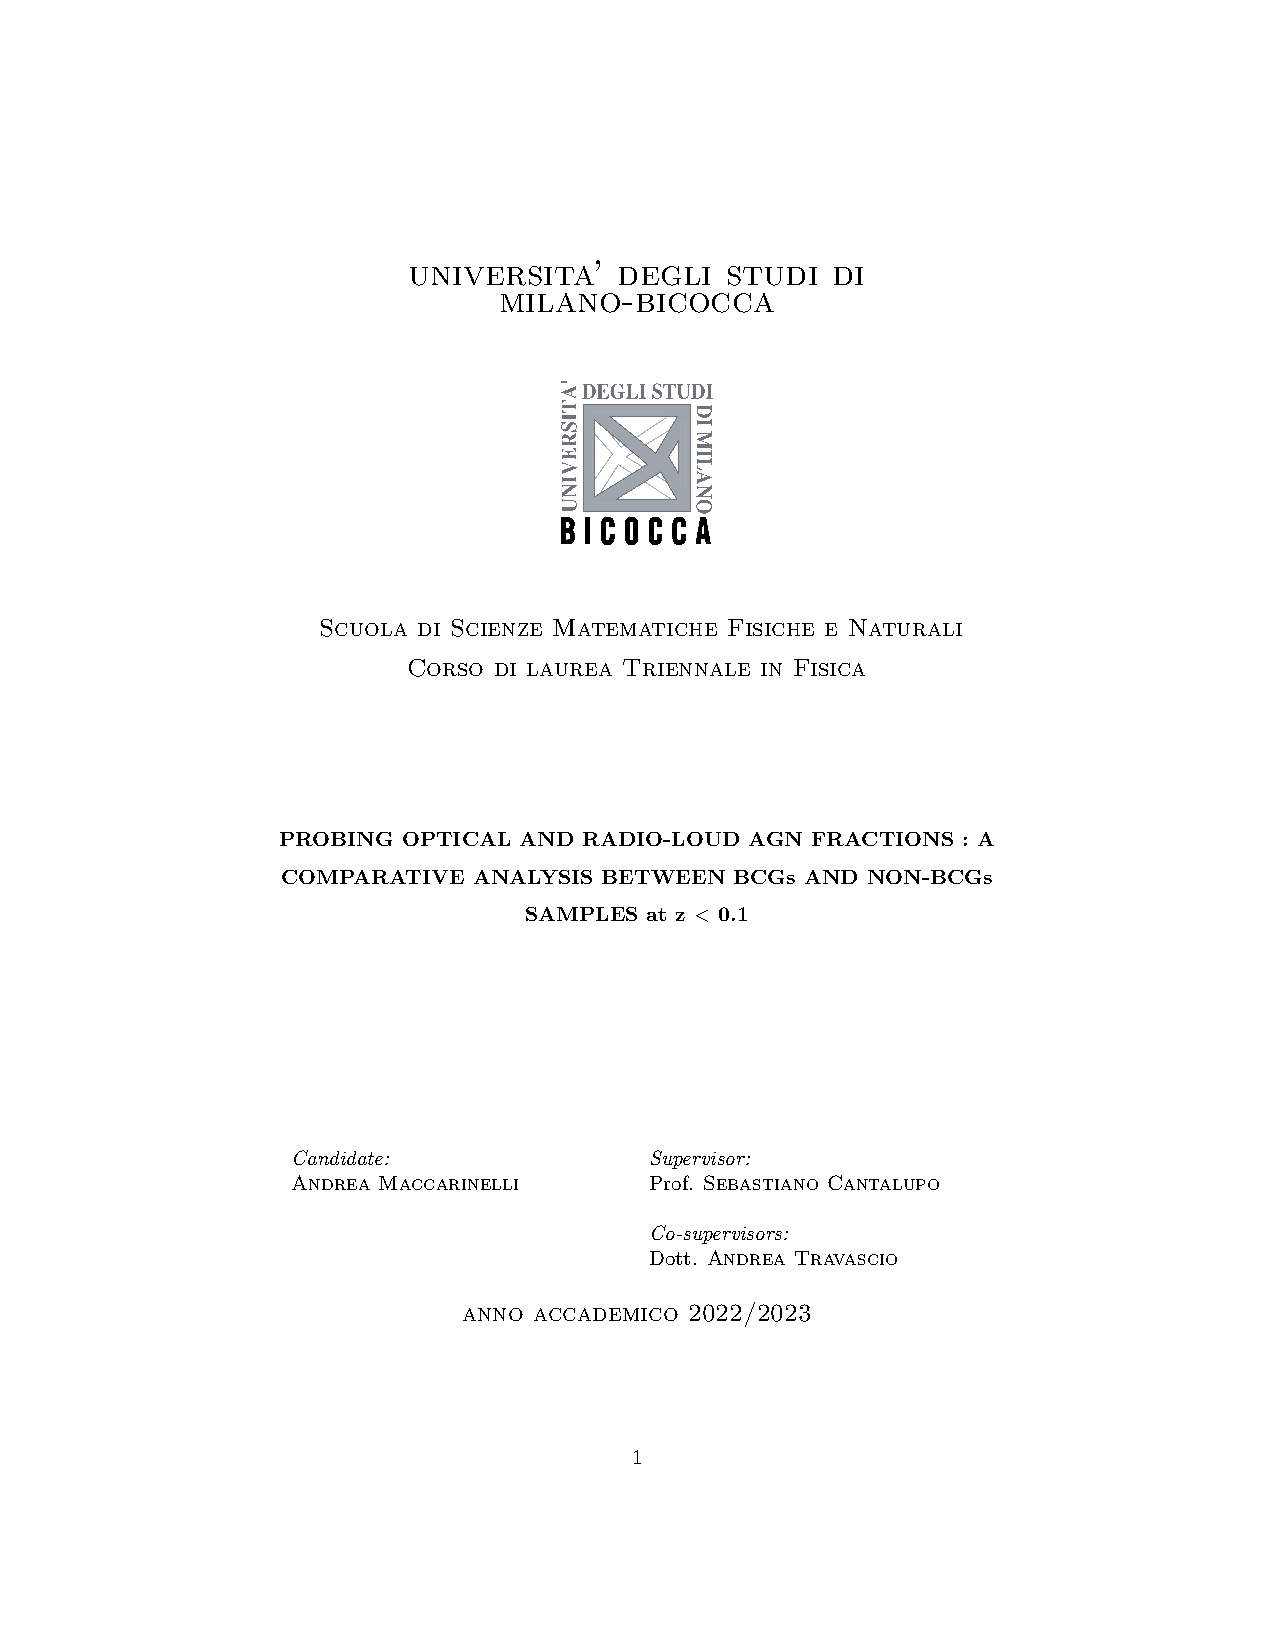
\includepdf{/Users/andreamaccarinelli/Desktop/BSc-ThesisRAW/frontespizio.pdf}
\include{Abstract}
\tableofcontents
\setcounter{page}{1}
\chapter{Introduction}

\section{The Active Galactic Nuclei: Quasar vs. Radio Accretion Modes}
Active galaxies constitute a distinctive class characterized by an intensely energetic source at their center, known as an Active Galactic Nucleus (AGN). Since the first observation of an active galaxy in the early 1900s \cite{Shields_1999}, numerous studies have been conducted on this intriguing category of galaxies. To this day, efforts persist in unraveling the nature and role of active galaxies within the broader context of galactic formation and evolution.

Research in this field has demonstrated that the intense radiation must emanate from a compact region, with a spatial dimension not exceeding 100 parsecs. This estimation was derived from the temporal variability observed in some of these sources \cite{1959ApJ...130...38W}. Additionally, it has been noted that AGNs exhibit luminosity variations of over $50\%$ within timescales ranging from days to years. Such fluctuations can only be explained if a substantial portion of the emission region is randomly connected. These observations strongly imply that the central component of AGNs is a rapidly accreting Supermassive Black Hole (SMBH).

AGN emissions span the entire electromagnetic spectrum, each wavelength band offers insights into specific components and associated phenomena within AGN \cite{2017NatAs...1E.194P}. 

In addition to the central SMBH \cite{2006ApJ...652..216R} there is a disk of accreting matter onto it, that emits a significant amounts of ultraviolet (UV) radiation. Above this disk, a cloud of relativistic electrons is believed to be there \cite{2005ASPC..343..435K}. This cloud reprocess the UV photons emitted from the disk, re-emitting them at X-ray energy levels.
A population of clouds exists in close proximity to the SMBH, that is known as the Broad Line Region
(BLR), because the kinematics of these clouds are significantly affected by the gravitational pull of the SMBH, resulting in broader spectral lines. Beyond the BLR, there exists an outer region surrounding the SMBH known as the Narrow Line Region (NLR). In contrast to the BLR, the NLR is characterized by narrower spectral lines, indicating distinct physical conditions and dynamics. 
Additionally, surrounding the disk, there's a toroidal-shaped volume composed of a mixture of gas and dust, leading to the partial absorption of central radiation. The torus is the main component used from the “Unified Model” \cite{1995PASP..107..803U} to explain the existence of different populations of AGN. According to this model, different AGNs are the same population of objects with specific inclinations to our line-of-sight direction \cite{1993ARA&A..31..473A}.

In particular we can distinguish:
 
\begin{itemize}
  \item \textbf{Type I:} For these types of AGN, broad emission lines, emitted from the BLR, with typical width in the range of in the range of $\sim 10^{3}$-$10^{4}$ $\text{km s}^{-1}$ exhibit a broad component,  along with narrow emission lines from the NLR. In this configuration, the observer is situated at a small angle relative to the torus axis, allowing the radiation from circumnuclear regions to remain unobscured along the line of sight.
  
  \item \textbf{Type II:} In this scenario, the spectrum of the AGN comprises solely narrow emission lines, not exceeding 1200 $  \text{km s}^{-1}$, due to the fact that the line of sight intersects the obscuring matter of the torus, obscuring the BLR.
  
\end{itemize}
A visual depiction of the Unified Model is shown in \autoref{2}.

The energy released during the accretion process of a SMBH plays a significant role in shaping the evolution of the host galaxy \cite{2021A&A...646A.167M}. In this context, the literature often discusses positive and negative feedback mechanisms.
Positive feedback occurring when the AGN feedback promotes stellar formation, while negative feedback involves the suppression of star formation, respectively. Feedback from SMBH accretion is capable of heating diffuse gas \cite{2005Natur.433..604D} and depositing heavy elements across the extensive surrounding environment \cite{2000ApJ...539L..13G}, with effects observed at scales exceeding kpc scales. Two distinct AGN feedback mechanisms have been proposed, each associated with different rates of mass accretion onto the SMBH (e.g. \cite{2012ARA&A..50..455F, 2017NatAs...1E.165H}).

\begin{itemize}
	\item \textbf{QSO's Radiative Feedback :} This feedback mode, often referred as quasar mode, consists in a high accretion rate of the SMBH via an optically-thick and geometrically-thin disk, and most of the energy is released in form of radiation.
	\item \textbf{QSO's Radio Feedback :} In this scenario, the SMBH accretion of hotter gas happens with a low rate in a optically-thin and geometrically-thick disk configuration, releasing energy in form of relativistic particles such as Radio Jets.
\end{itemize}
%Check ok !!!
\begin{figure}[hbtb]
  \centering
  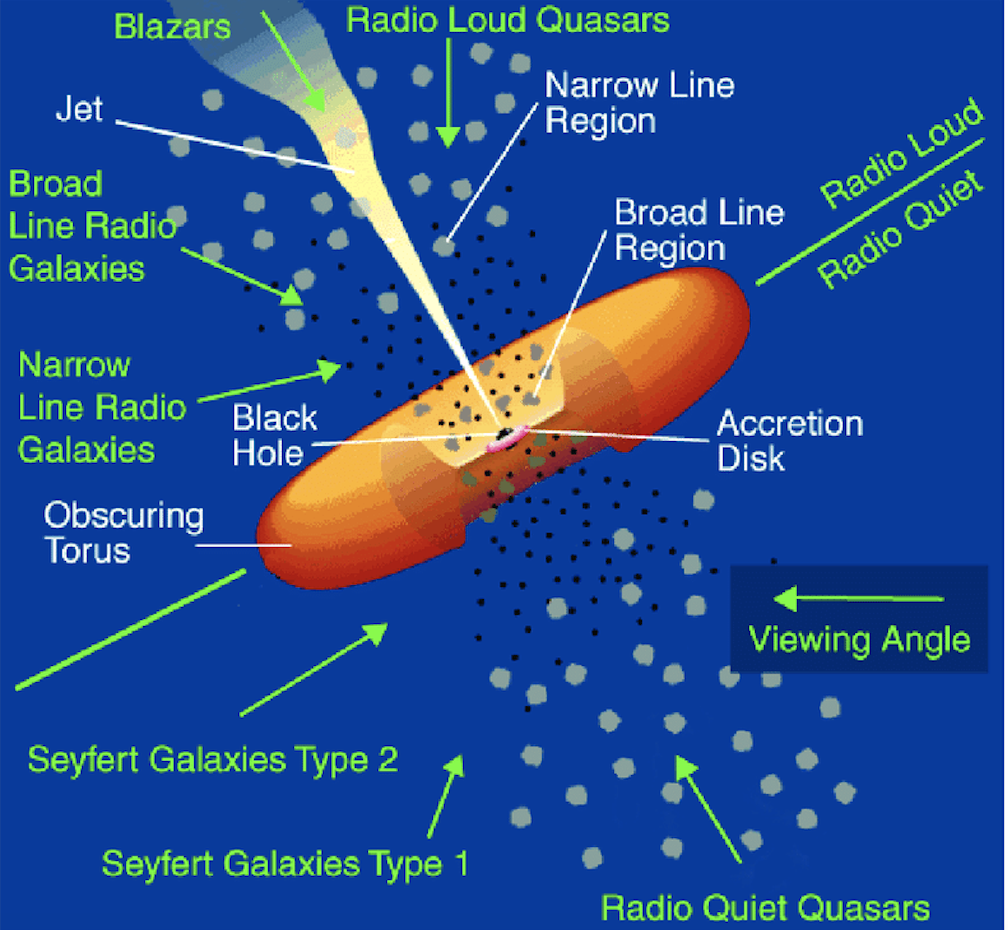
\includegraphics[width=0.5\textwidth]{UnifiedAGNmodel}
  \caption{The Unified AGN model as proposed in \cite{1995PASP..107..803U}, It elucidates AGN taxonomy by considering various viewing angles relative to the torus.}
  \label{2}
\end{figure}

\section{The Brightest Cluster Galaxies }
The Hierarchical Galaxy Formation Model stands as a cornerstone in our understanding of cosmic structure formation, delineating the principal pathways through which galaxies growth their stellar and gas mass assimilating matter from their surroundings \cite{1994MNRAS.271..781C}.

One of the most extreme examples in this context involves the study of Brightest Cluster Galaxies (BCGs), a unique class of galaxies, situated at the center and typically standing out as the most luminous and massive objects within the entire cluster.( e.g. \cite{2015MNRAS.448....2W} ). Considering their environment, observational studies, have indicated that the evolution of BCGs differs from the normal galactic path \cite{2020MNRAS.498.2719T}. As different studies have shown, BCGs' mass assembly is primarily influenced by dry mergers \cite{2007MNRAS.375....2D, 2019ApJ...881..150C}.

The majority of the BCGs are elliptical galaxies, but their properties deviate from established scaling relations for ellipticals. While most BCGs align with the Fundamental Plane, deviations, such as lower velocity dispersions and larger radii than predicted by the Faber–Jackson and Kormendy relations, have been observed (e.g \cite{1991ApJ...375...15O}). Recent findings suggest variations in these relations based on galaxy luminosity for all ellipticals. Additionally, BCG surface brightness profiles and radii depend on host cluster properties \cite{2005MNRAS.364.1354B}. 

\begin{comment}
Due to their distinct evolutionary histories, the primary mechanism driving the mass growth of galaxies is associated with cooling flows within lower mass halos at high redshifts.
However, at low redshifts, this phenomenon diminishes, primarily due to increased Active Galactic Nuclei ( AGN ) activity accreting mass into their typically hosted SMBH \cite{2006ApJ...652..216R}.
 \end{comment}
 
BCGs are mainly characterized by Radio Mode accretion of their SMBH, thus exhibiting radio loud emission as well as radio jets. As presented in \cite{2007MNRAS.379..867V} these relativistic jets of radio emission are also recognized as one of the main explanation of the so called "Cooling flow problem". 
While Theoretical expectations propose rapid cooling and gas flow toward the center, fostering new star formation, actual observations reveal a much slower cooling process, leading to the discrepancies.
The inclusion of radio jets provides a resolution to this issue by infusing energy into the Intracluster Medium (ICM), the hot gas within a galaxy cluster. This injection hinders the rapid cooling and collapse of gas toward the center, deviating from theoretical predictions. However observational studies found that temperature of cluster cores fails to fall below $\sim 30\%$ at large radii resulting in an amount of cooling gas corresponding only to the $\sim 10\%$ expected from the existent cooling flow model. \cite{David_2001} % OKOKOK

\newpage
\section{ Main Scientific Question of the Thesis} %Chiedere come mai ci distanziamo così tanto dalle scorse tesi
In this context, the main scientific question driving this work is to understand \textbf{whether the special evolution of BCGs, along with their dense environment, affects the accretion of SMBHs in their centers compared to other types of galaxies in the local universe}.

In particular, this study will present a comparative analysis between two representative samples of BCGs and Non-BCGs to highlight the substantial differences that the cluster environment induces in SMBH accretion.


To address this particular question, I conducted an analysis on a galaxy sample, the Sloan Digital Sky Survey Data Release 7 (SDSS DR7), as outlined in \cite{2009ApJS..182..543A}, and the C4 BCGs catalogue by Anja Von Der Linden and Best \cite{2007MNRAS.379..867V}. For these specific BCGs and non-BCGs sample, I utilized the common optical line fluxes ($H\alpha$, [OIII], $H\beta$, [NII], and [SII] doublets) provided by the Max Planck Institute for Astrophysics and Johns Hopkins University team to classify the galaxies hosting an AGN on the basis of the standard optical diagnostic diagram known as BPT \cite{1981PASP...93....5B}. Furthermore, through the cross-match between the aforementioned catalogs with datasets derived from NVSS and FIRST radio surveys, as outlined in \cite{2005MNRAS.362....9B}, I identified BCGs associated with radio loud emission, as an indication of the presence of radio mode SMBH accretion and a potential radio jet.

The analyses and the description of the data will be presented in the next chapter. 

%%%%% Apparentemente tutto corretto secondo le correzioni di Andrea 
    
\chapter{Methods}
In this thesis, I analyze a dataset comprising the properties of a sample of galaxies from the Seventh Data Release (DR7) of the Sloan Digital Sky Survey. Covering 11,663 square degrees of imaging data, DR7 offers extensive five-band photometry for 357 million celestial objects \cite{2009ApJS..182..543A,mpa-sdss-dr7}. 

As shown in  Fig.\ref{3}, the Legacy imaging footprint is depicted as the extensive contiguous gray area on the left side of the upper panel, complemented by three separated gray stripes visible on the right side.

With completed spectroscopy over 9380 square degrees, including 1.6 million spectra of galaxies, quasars, and stars, the SDSS DR7 dataset serves as the primary catalog for this study. A depiction of the spectroscopic coverage is shown in the lower panel of Fig.\ref{3} .
 
I will focus on following physical properties : \textbf{Redshift} and \textbf{Integrated flux with their relative uncertainties} of the common optical lines (i.e. $H\alpha$, $H\beta$...).

In the context of SDSS DR7, these properties are calculated using an automated procedure of gaussian fitting, applied in two subsequent moments. In the first phase the object is classified and redshift is calculated by fitting at the same moment only the emission lines, while in the second part of the procedure this computation is extended to all lines available. It is important to note that \textbf{each} line is \textbf{individually fitted as a single Gaussian} on the continuum-subtracted spectrum, with modalities presented by O'Donnell \cite{1994ApJ...422..158O}. Information on the Radio classification of the galaxies in this sample is obtained from FIRST and NVSS images from Best et Al. \cite{2005MNRAS.362....9B}.

\begin{comment}
the line-fitting process is divided into three main stages during an automated Gaussian fitting procedure applied to continuum subtracted data as
\begin{enumerate}
\item The first stage involves fitting to only emission lines, referred to as "foundLines," and is performed during the determination of emission line redshifts.

\item The second stage, termed "measuredLines," represents the final fitting of all lines, including both emission and absorption lines. This stage occurs after the object has been classified, and the redshift has been determined.
\end{enumerate}
It is important to note that \textbf{each} line is \textbf{individually fitted as a single Gaussian} on the continuum-subtracted spectrum, with modalities shown in \cite{1994ApJ...422..158O}.
\end{comment}

%FINO A QUI SOPRA SEMBRA OK 
 
%COMMENTI DI ANDREA
 \begin{comment}
 Specifically, I will focus on…. 


BREVEMENTE:
devi dire che utilizzi le seguenti proprietà: 
integrated flux and relative uncertainties of the common optical emission lines, i.e.,,,
(spiega come sono state derivate)
,redshifts (spiega con quale riga sono stati derivati)

Il redshift è lo shift verso il rosso dovuto perlopiù all’espansione dell’universo.
Si calcola solitamente avendo la lambda della riga osservata (lamb_obs), la lambda della riga osservata in laboratorio, quindi aspettata dalla teoria (lamb_exp) e si calcola come:

z = (lamb_obs/lamb_exp) -1

solitamente si usano righe come l’Hbeta o Halpha stretto. Ancora meglio righe molecolari. Vedi che hanno usato loro e dillo-.

Poi dì anche che sfrutterai informazioni fotometriche nel radio.

comunque andrai a parlarne dopo nel dettaglio 
\end{comment}
%VERSIONE INIZIALE CHE AVEVO MESSO IO
\begin{comment}
The study of cosmic objects, such as galaxies, relies on the analysis of the electromagnetic spectrum emanating from these distant sources. Within a spectrum, various pieces of information can be extracted, with the primary focus being on the intensity of light across a range of energies or frequencies. A crucial aspect of a spectrum involves determining the intensity at specific wavelengths.

This thesis will concentrate on utilizing specific information derived from spectra (e.g., flux, flux error) associated with both permitted and forbidden emission lines. In a galactic context, particularly within a galaxy cluster, the continuum originates from the diffuse light emitted by stars. On the other hand, emission lines, which are prominently observed in such environments, are typically generated by elements like Hydrogen, Helium, Oxygen, etc.

There are various methods to investigate the electromagnetic spectrum, with the two primary branches being Spectroscopy and Photometry.

Astrophysical spectroscopy is a fundamental tool used to analyze the electromagnetic radiation emitted or absorbed by celestial objects. By examining the spectral lines and features, it is possible to mine important informations such as chemical composition, temperature, density etc.

On the other hand, photometry measures the overall brightness of celestial objects across different wavelength bands, providing information about the spectral distribution of their luminous emission. 

In this Thesis Work i'll be focusing on a Spectroscopic study involving the fluxes of the Forbidden Emission lines of the spectrum.
\end{comment}



%CAPITOLO DESCRIZIONE DEI SAMPLE UTILIZZATI
\section{Data Description}
This thesis presents results obtained through the cross-matching of three distinct celestial catalogues:
\begin{itemize}
	\item\textbf{SDSS DR7 :}  Main Catalogue of galaxies \cite{2009ApJS..182..543A,mpa-sdss-dr7}
	\item \textbf{C4-BCG :}  BCG Catalog \cite{2009yCat..73790867V}
	\item \textbf{Best at Al. :}   Survey for RadioLoud identification \cite{2005MNRAS.362....9B}
\end{itemize}

\subsection{SDSS DR7}
The Sloan Digital Sky Survey (SDSS) project, is a comprehensive astronomical survey that maps the universe by capturing images, spectra, and photometric data of celestial objects over a large area of the sky, with a spectroscopic footprint area of 9'380 \text{$deg^2$} and an imaging surface covered of  11'663 \text{$deg^2$} \cite{2009ApJS..182..543A} as shown in Fig.\ref{3}.

Observations have been conducted using a a dedicated wide-field 2.5 m telescope \cite{2006AJ....131.2332G} located at Apache Point Observatory (APO) near Sacramento Peak in Southern New Mexico. The telescope employs two distinct instruments, making possible both Imaging and Spectroscopy measures. First measurements are carried out with a wide field imager composed by 24x 2048 × 2048 CCDs on the focal plane \cite{1998AJ....116.3040G}.
This photometric system comprises five color bands (u, g, r, i, and z) that divide the entire range from the atmospheric UV cutoff at 3000 $\AA$ to the sensitivity limit of silicon CCDs at 11000  $\AA$ into five essentially non overlapping passbands.

Spectroscopic measurements are carried out with a pair of multiobject double spectrographs, receiving the light from 640 optical fibers, each of the spectrographs cover a wavelength range from 3800 $\AA$ to 9200 $\AA$ with a spectral resolution of $\frac{\lambda}{\Delta \lambda} \approx 2000$. \cite{2009ApJS..182..543A}
\vspace{0.5cm}

In this thesis, I work with a dataset of properties estimated by the Max Planck Institute for Astrophysics and Johns Hopkins University (MPA-JHU) team for a total of 927,552 galaxies belonging to the Sloan Digital Sky Survey Data Release 7 (SDSS DR7) \cite{2009ApJS..182..543A, mpa-sdss-dr7}.

The main Physical Properties of interest for this study are \textbf{Redshift} and \textbf{Integrated flux with relative uncertainty} for common optical lines (i.e., $H\alpha$, $H\beta$, [N II]6584, [O III]5007, [S II]6731, [S II]6716).

These properties resulted from calculations of two automated spectroscopic pipelines : \textit{spectro2d} and \textit{spectro1d} \cite{2002AJ....123..485S}.

 These pipeline analyzes combined spectra informations, determining object classifications and initial redshifts. Emission and absorption redshifts are independently measured for each object to avoid biases.

Emission line redshifts are then determined by identifying lines through wavelet transform and performing Gaussian fits.
The redshift that I use in this thesis is based on the best-fit model of absorption and emission lines. 

\begin{comment}
The spectroscopic pipelines, \textit{spectro2d} and \textit{spectro1d}, process two-dimensional spectrograms from the spectrographs, converting them into flux- and wavelength-calibrated spectra. These pipelines also handle the measurement of emission and absorption features, classification of spectra, and redshift determination. The \textit{spectro2d} pipeline reduces raw data from red and blue CCD cameras, producing merged, calibrated spectra for analysis by \textit{spectro1d}. All wavelengths are given in angstroms, vacuum-corrected to the heliocentric frame, with flux density in units of $10^{-17} \, \text{ergs} \, \text{cm}^{-2} \, \text{s}^{-1} \, \text{\AA}^{-1}$.

The \textit{spectro1d} pipeline classifies spectra, determines emission and absorption redshifts, and measures lines. The specObj class contains parameters for the entire spectrum, including links to plate information, PhotoObj data, and related objects in SpecLine, SpecLineName, SpecLineIndex, CrossCorrelationRedshift, and EmissionRedshift tables. The pipeline also provides flux- and wavelength-calibrated spectra, continuum-subtracted spectra, 1 sigma error estimates per pixel, and mask arrays.

State and warning bits are assigned for the redshift, and objects are classified based on redshift and other features.
\end{comment}

\begin{comment}
The main Physical Properties of Interest for our study are \textbf{Redshift} and \textbf{Integrated flux with relative uncertainty} regarding common optical lines (i.e. $H\alpha$, $H\beta$, also including molecular lines (i.e.  [N II]6584, [O III]5007, [S II]6731 [S II]6716]). 

The spectroscopic pipelines , \textit{spectro2d} and \textit{spectro2d}, process two-dimensional spectrograms from the spectrographs, converting them into flux- and wavelength-calibrated spectra. These pipelines also handle the measurement of emission and absorption features, classification of spectra, and redshift determination. The \textit{spectro2d} pipeline reduces raw data from red and blue CCD cameras, producing merged, calibrated spectra for analysis by \textit{spectro2d}. All wavelengths are given in angstroms, vacuum-corrected to the heliocentric frame, with flux density in units of $10^{-17} \, \text{ergs} \, \text{cm}^{-2} \, \text{s}^{-1} \, \text{A}^{-1}$.

The \textit{spectro1d} pipeline classifies spectra, determines emission and absorption redshifts, and measures lines. The specObj class contains parameters for the entire spectrum, including links to plate information, PhotoObj data, and related objects in SpecLine, SpecLineName, SpecLineIndex, CrossCorrelationRedshift, and EmissionRedshift tables. The pipeline also provides flux- and wavelength-calibrated spectra, continuum-subtracted spectra, 1 sigma error estimates per pixel, and mask arrays.

The redshift calculation in the \textit{spectro2d} pipeline involves several distinct steps. Firstly, the pipeline analyzes combined spectra, determining object classifications and initial redshifts. This includes measurements of spectral lines and warning indicators. Emission and absorption redshifts are independently measured for each object to avoid biases.

Continuum subtraction follows, where a fifth-order polynomial is used, and the fitted continuum is subtracted from the spectrum. Emission line redshifts are then determined by identifying lines through wavelet transform and performing Gaussian fits. The final emission-line redshift is chosen based on the highest confidence level.

Spectra are cross-correlated with stellar, emission-line galaxy, and quasar templates to obtain cross-correlation redshifts. The redshift with the highest confidence level among all templates is chosen as the cross-correlation redshift.

The final redshift is determined by choosing the highest confidence level between emission and cross-correlation redshifts. State and warning bits are assigned for the redshift, and objects are classified based on redshift and other features.
\end{comment}

%\vspace{1.5cm}
\begin{figure}[hbtp]
  \centering
  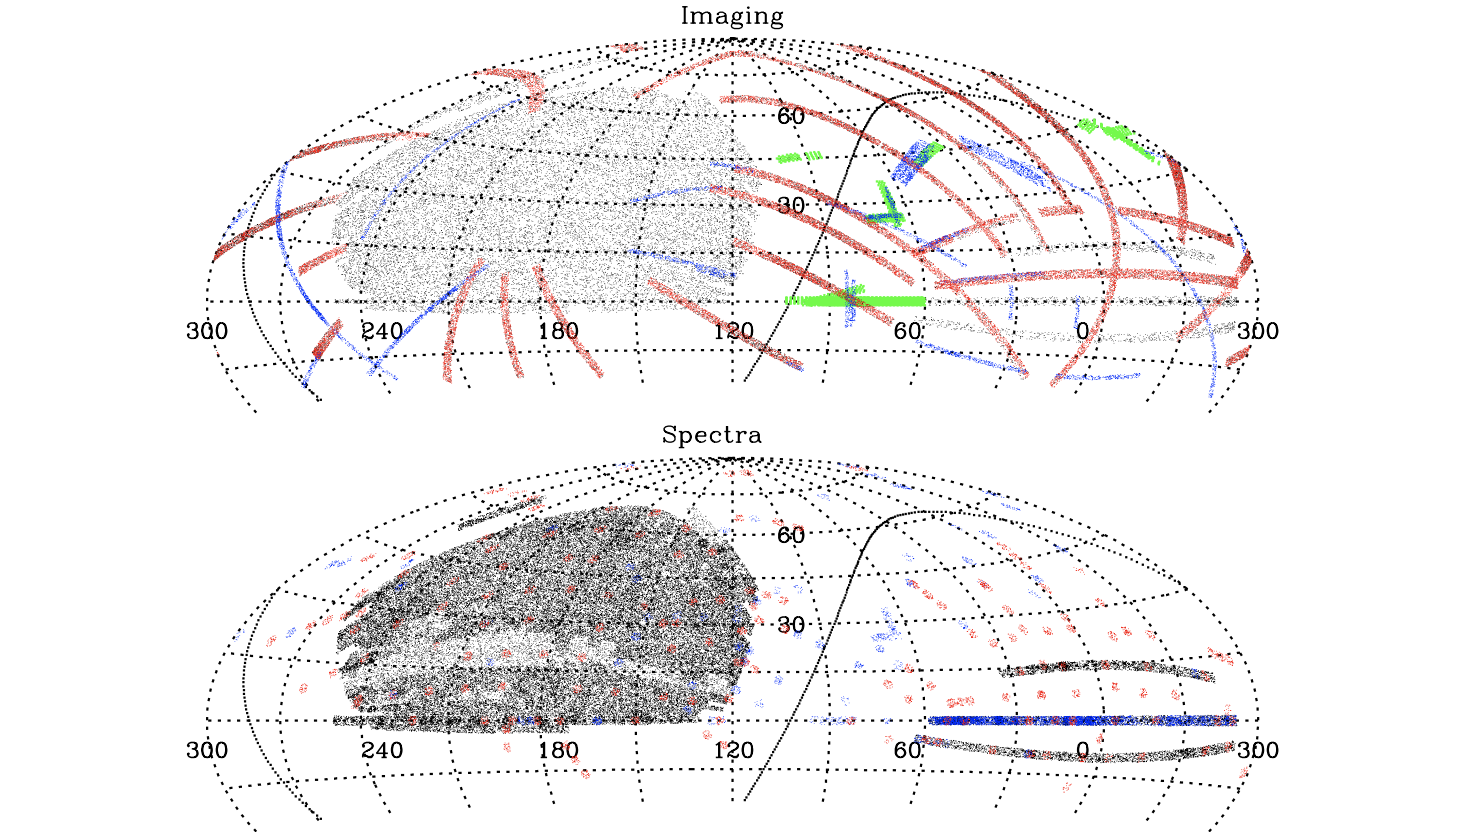
\includegraphics[width=1\textwidth]{SDSS_OFF}
  \caption{Distribution on the sky of the data included in DR7 (upper panel: imaging; lower panel: spectra), shown in an Aitoff equal-area projection in J2000 Equatorial Coordinates. The Galactic plane is the sinuous line that goes through each panel. \cite{2009ApJS..182..543A}}
  \label{3}
\end{figure}


\begin{comment}
 The first is a wide-field imager equipped with 24 tiles, each containing a 2048x2048 CCD. Imaging is performed along great circles at the sidereal rate, leading to exposure times of 54.1 seconds.

The astrometry is good to 45 milliarcseconds (mas) rms per coordinate at the bright end, while the photometric calibration is made in two modalities, respectively by tying to standard reference stars and by using the overlap between adjacent imaging runs in a process called ubercalibration.

Spectra are extracted and calibrated in terms of wavelength and flux. For galaxies near the main sample flux limit, the typical signal-to-noise ratio (S/N) is 10 per pixel. The broadband spectrophotometric calibration exhibits an accuracy of $4\%$ root mean square (rms) for point sources (Adelman-McCarthy et al. 2008), and the wavelength calibration is precise to $2 \, \text{km s}^{-1}$.

The SDSS data have been made public in a series of yearly data releases, This thesis works based its results from a galactic sample derived from "Data Release 7" by the Max Planck Institute for Astrophysics and Johns Hopkins University ( MPA-JHU )  teams, containing the derived properties of a total of 927'552 galaxy spectra.


\textbf{Physical Properties of interest :}
\begin{itemize}
		\item \textbf{Line Flux :}Flux from Gaussian fit to continuum subtracted data, corrected for foreground (galactic) reddening using techniques developed by O'Donnell \cite{1994ApJ...422..158O}
		\item \textbf{Error Line Flux :} Developed by analyzing the duplicate observations of galaxies, to compare the empirical spread in value determinations with the random errors.

\end{itemize}

\end{comment}


\subsection{C4 BCG Catalogue}
The identification of BCGs within the primary galaxy sample, previously described, relies on the BCG catalogue created by A. Von der Linden et al. \cite{2007MNRAS.379..867V, 2009yCat..73790867V}. This sample is derived from the further analysis of the C4 Galaxy Cluster Catalog,  developed by Miller et Al.  \cite{2005AJ....130..968M}.

The C4 catalog comprises 1106 galaxy clusters identified in the Third Data Release (DR3) of SDSS spanning redshifts from 0.02 to 0.16. 

In this context, the work by Von Der Linden et al.  \cite{2007MNRAS.379..867V} is noteworthy, as it builds upon the C4 catalog but introduces improved procedures for BCG identification and cluster velocity dispersion measurements, ultimately yielding a sample of 625 BCGs.

Despite primarily serving as a cluster catalogue, the original C4 also offered potential BCG candidates by identifying both a \textit{spectroscopic} candidate and a \textit{mean} candidate within each cluster. However, subsequent research conducted by Von Der Linden et al. revealed that approximately $30\%$ of identified clusters missed the true BCG due to fiber collisions in the SDSS spectrometry.
To address this issue and to construct a specific BCG sample, Von der Linden's team initially limited the sample by imposing $z\leq 0.1$ in order to ensure that clusters span a large angular extent in comparison to the minimum distance between SDSS spectrometry fibres of $\sim55$ arcsec. 
At this redshift, the magnitude limit in the red band of the spectroscopic sample is approximately $M_{r} \approx -20$, encompassing an initial sample of 833 clusters. The subsequent selection process involved a specific procedure including the estimation of the virial radius, the selection of the two brightest galaxies within the projection of the mean galaxy, and the application of criteria such as the concentration index and redshift/color compatibility for the final BCG identification.
Throughout the computation, several galaxies were lost due to two main structural reasons : initial misclassification of stars and associations with multiple clusters. This led to the rejection of more than 101 clusters, leading to the final sample of 625 elements.



\subsection{The Radio Catalogue}

I also exploit the radio catalog obtained from Best et al., containing 2712 radio sources selected as Radio loud and star-forming \cite{2005MNRAS.362....9B}. In order to study the fraction of the “BCG” and “non-BCG” samples it has been necessary to cross-match this catalog with that obtained from the match between SDSS and C4 in the previous section.
The Authors created this survey from the cross-match of a main spectroscopic galaxy sample and two radio surveys: the National Radio Astronomy Observatories (NRAO) Very Large Array (VLA) Sky Survey (NVSS) \cite{1998AJ....115.1693C} and the Faint Images of the Radio Sky at Twenty centimeters (FIRST) \cite{1995ApJ...450..559B}.


The NVSS was the first radio survey with an angular resolution of 45 arcsec. 
The FIRST catalogue offers angular resolution of 5 arcsec. Nonetheless, the high angular resolution of FIRST presents its own challenges, as it is insensitive to extended radio structures and resolves out the extended emission of radio sources. Consequently, the total radio luminosity of sources larger than a few arcseconds is systematically underestimated by FIRST. To address these limitations, a hybrid approach utilizing both NVSS and FIRST surveys has been developed to identify radio sources associated with galaxies in the SDSS spectroscopic sample. This approach capitalizes on the sensitivity of NVSS to large-scale radio structures and the high angular resolution of FIRST to reliably pinpoint the host galaxy.

The obtained radio source sample demonstrated a completeness of $95\%$ and a reliability of $98.9\%$, upgrading the achievable performance of each individual survey. The sample was subsequently classified into two groups: radio-loud active galactic nuclei (AGN) and galaxies where radio emission is predominantly driven by star formation. Classification was based on galaxies' positions in the plane of 4000 $\AA$ break strength versus radio luminosity per unit stellar mass, resulting in a dataset of 2,215 radio-loud AGN and 497 star-forming galaxies with radio luminosity exceeding 5 mJy at 1.4 GHz. \cite{2005MNRAS.362....9B, 10.1111/j.1365-2966.2005.09192.x}



\begin{comment}
This catalog is used to investigate the presence of radio counterpart of BCG and normal galaxies in the main SDSS catalogue, therefore, this is cross-matched with a main spectroscopic galaxy sample and two radio surveys: the National Radio Astronomy Observatories (NRAO) Very Large Array (VLA) Sky Survey (NVSS) \cite{1998AJ....115.1693C} and the Faint Images of the Radio Sky at Twenty centimeters (FIRST) survey \cite{1995ApJ...450..559B}.
\end{comment}


\begin{comment}
To investigate the radio emission characteristics of both BCGs and non-BCGs, this study conducted a crossmatch between the primary SDSS sample and a dataset comprising 2,712 radio-luminous galaxies from the work by \cite{2005MNRAS.362....9B}. This collection of radio-luminous objects resulted from a complex cross-matching process involving the main spectroscopic galaxy sample and two radio surveys: the National Radio Astronomy Observatories (NRAO) Very Large Array (VLA) Sky Survey (NVSS) \cite{1998AJ....115.1693C} and the Faint Images of the Radio Sky at Twenty centimeters (FIRST) survey. \cite{1995ApJ...450..559B}

The NVSS was the first radio survey with a sufficiently high angular resolution (45 arcsec) to allow automated cross-correlation with optical surveys. However, the FIRST catalogue offers superior angular resolution (approximately 5 arcsec), resulting in samples with much higher reliability. Nonetheless, the high angular resolution of FIRST presents its own challenges, as it is insensitive to extended radio structures and resolves out the extended emission of radio sources. Consequently, the total radio luminosity of sources larger than a few arcseconds is systematically underestimated by FIRST. To address these limitations, a hybrid approach utilizing both NVSS and FIRST surveys has been developed to identify radio sources associated with galaxies in the SDSS spectroscopic sample. This approach capitalizes on the sensitivity of NVSS to large-scale radio structures and the high angular resolution of FIRST to reliably pinpoint the host galaxy.

The obtained radio source sample demonstrated a completeness of $95\%$ and a reliability of $98.9\%$, upgrading the achievable performance of each individual survey. The sample was subsequently classified into two groups: radio-loud active galactic nuclei (AGN) and galaxies where radio emission is predominantly driven by star formation. Classification was based on a galaxy's position in the 4000-Å break strength versus radio luminosity per unit stellar mass plane, resulting in a dataset of 2,215 radio-loud AGN and 497 star-forming galaxies with radio luminosity exceeding 5 mJy at 1.4 GHz.
\end{comment}

\newpage
\section{Data Analysis}
The initial step of the analysis involved cross-matching the catalog of galaxy properties from the MPA-JHU emission line analysis for the SDSS DR7 with the C4 BCG sample, presented in the previous chapter, in order to identify the BCG candidates. In particular, using coordinates of the galaxies in both these samples, I selected galaxies in the SDSS catalog closest to the individual BCGs in the C4 catalog, within a distance of less than 2 arcseconds (i.e. the PSF of 1.4 arcsec). 
A distinct catalog was created for galaxies selected as “non-BCG”, which were exclusively chosen from within the cross-matched region of these surveys to minimize contamination from BCGs not included in the C4 catalog. 

At the end, through this process, i obtained two distinct samples, each containing comprehensive spectral properties for a total of 404 and 389454 galaxies identified as BCG and non-BCG, respectively. 
In Fig.\ref{Cross:SDSS/C4} I report the distribution of galaxies from SDSS DR7 in grey and the BCGs identified from the crossmatch in red. The black dashed squares show the cross-matched area used to produce the BCG and non-BCG samples.

\begin{figure}[hbtp]
  \centering
  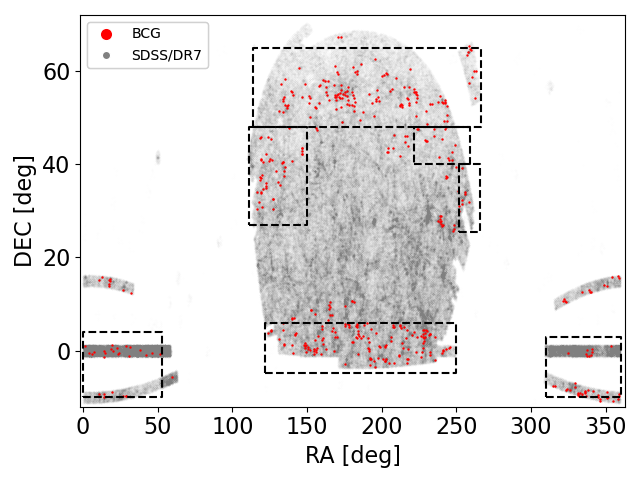
\includegraphics[width=0.8\textwidth]{BCGcmSDSS}
  \caption{Distribution of data on the sky in J2000 Equatorial Coordinates. The grey areas represent galaxies included in the main sample \cite{mpa-sdss-dr7}, while BCGs identified through crossmatching are highlighted in red. Dashed lines delineate the regions used for constructing the non-BCG sample. }
  \label{Cross:SDSS/C4}
\end{figure}

The final step in radio identification involves identifying galaxies exhibiting radio loud emission within both the BCG and non-BCG samples. This additional crossmatching process led to a refinement of the spatial regions, ensuring greater precision in excluding galaxies that may exhibit radio loudness but are not relevant to the radio survey under study.


%% LA PARTE CHE AVEVO SCRITTO IO SULL'INTRODUZIONE AI DATI
\begin{comment}
As previously introduced, our primary galaxy sample for astrometry measurements is the MPA-JHU SDSS-derived catalogue.

The first operation required for the development of our study involved crossmatching the C4 BCG sample \cite{2009yCat..73790867V} to extract data files from the main sample, including both BCGs and non-BCGs.

This initial crossmatch was accomplished by selecting the nearest element within a radius of 2 arcsec in both RA and Dec corresponding to each of the BCGs in \cite{2009yCat..73790867V}. The result was a list of 484 corresponding selected elements.

At the end of this initial phase, the following data were collected for both samples:
\begin{itemize}
    \item \textbf{Astrometry data:} Celestial coordinates, Redshift, Error on redshift...
    \item \textbf{Spectroscopy measures:} Emission lines' fluxes and their relative errors
\end{itemize}
Even though further explanation is to follow, it is preferable to introduce the second crossmatch required for this work, this time with the 2712 galaxy samples of Celestial Objects found to be active in the radio field.

In this case, the research algorithm was designed to identify the nearest correspondence within a radius of 5 arcsec. The previously created files were appropriately updated by adding a specific flag, denoted as 1, to indicate whether, when found in the Radio Sample, it implies Radio Loud Emission.
\end{comment}



\subsection{Optical AGN Identification via BPT Diagram in BCG and non-BCG Samples}
In this section, we present an analysis aimed at detecting AGN activity within the galaxies in both the "BCG" and "non-BCG" samples.
To do it we use the Baldwin, Phillips $\&$ Terlevich (BPT) diagnostic diagram \cite{1981PASP...93....5B}.
This analysis is widely performed in literature to classify various types of galaxies based on the ratio of certain optical emission lines emitted from the gas within the host-galaxy, known as the inter-stellar medium (ISM). According to photoionization models, these line ratios are significantly influenced by the properties of the gas and its ionization level.
These specific ratios have been carefully chosen to prioritize similar wavelength fractions, minimizing dust attenuation. Specifically, this is developed based on the following ratios: $([OIII]\lambda 5007/H\beta), ([NII]\lambda 6583/H\alpha), ([SII]\lambda\lambda 6716,6731 / H\alpha), ([OI]\lambda 6300 / H\alpha)$.

While the ideal classification incorporates all three primary BPT diagnostics, this study relies on a classification derived solely from the BPT diagrams for [NII] and [SII], based on the plot of $[OIII]\lambda 5007/H\beta$ versus  $[NII]\lambda 6583/H\alpha$ and $[OIII]\lambda 5007/H\beta$ versus $[SII]\lambda\lambda 6716,6731 / H\alpha$, respectively.

%\newpage
According to different photoionization models, demarcation lines can be drawn for the purpose to classify galaxies into different categories \cite{2006MNRAS.372..961K}. Specifically, galaxies are classified into AGN, Composite, and Star Forming in the BPT-[NII] diagram, and as Seyferts, LINERs, and Star Forming in the BPT-[SII] diagram. I provide an explanation of the nature of the different categories to follow:


 %in the BPT-[NII] diagram, the categories include AGN, Composite, and Star Forming while in the BPT-[SII] diagram, the populations are Seyferts, LINERs, and Star Forming Galaxies.

%\begin{itemize}
    %\item \textbf{BPT-[NII]:}
		\begin{itemize}
    		 \item \textbf{AGN:} Galaxies dominating the upper-right part of the diagram are characterized by high [NII]/H$\alpha$ and [OIII]/$H\beta$ ratios suggesting that non-stellar processes play a crucial role in ionization.
		  \item \textbf{Composite:} The intermediate region between star-forming and AGN-dominated areas is occupied by galaxies that show a combination of both star formation and AGN activity. Emission line ratios, including [NII]/H$\alpha$ and [OIII]/H$\beta$, fall in intermediate ranges compared to pure star-forming or AGN-dominated regions.
		%\item \textbf{Star-forming (SF):} Galaxies residing in the lower-left portion of the diagram are primarily powered by ongoing star formation. These regions exhibit low [NII]/H$\alpha$ and [OIII]/H$\beta$ ratios, indicating the dominance of ionization processes related to massive stars.

		\end{itemize}

		 %\item \textbf{BPT-[SII]:}
		\begin{itemize}
    		\item \textbf{Seyferts:} The upper-right portion of the diagram is dominated by galaxies with high [SII]/H$\alpha$ and [OIII]/H$\beta$ ratios meaning strong non-stellar ionization processes.
    		\item \textbf{LINERs (Low-Ionization Nuclear Emission-line Regions):} The intermediate region between star-forming and Seyfert areas is populated by galaxies exhibiting low-ionization emission lines in their nuclei. This suggests a presence of weak AGN activity with low [OIII]/H$\beta$ and intermediate [SII]/H$\alpha$ ratios.
		 \item \textbf{Star-forming :} Galaxies situated in the lower-left region of the diagram are primarily influenced by ongoing star formation. Emission line ratios, such as low [NII]/H$\alpha$ or [SII]/H$\alpha$ and [OIII]/H$\beta$, indicate ionization predominantly driven by massive stars.
		\end{itemize}

%\end{itemize}

The classification via BPT diagnostic diagrams is based on the demarcation functions presented in Kewley et al 2006 \cite{2006MNRAS.372..961K}, that are outlined to follow:
\begin{itemize}
    \item \textbf{BPT-[NII] Demarcation Functions:}
    \begin{itemize}
        \item Kauffmann+03 Line: \[ \text{log}(\frac{\text{[OIII]}}{\text{H}\beta}) = 0.61 / (\text{log}(\frac{\text{[NII]}}{\text{H}\alpha}) - 0.05) + 1.3 \]
        \item Kewley+01 Line: \[ \text{log}(\frac{\text{[OIII]}}{\text{H}\beta}) = 0.61 / (\text{log}(\frac{\text{[NII]}}{\text{H}\alpha}) - 0.47) + 1.19 \]
    \end{itemize}

    \item \textbf{BPT-[SII] Demarcation Functions:}
    \begin{itemize}
        \item Main AGN Line: \[ \text{log}(\frac{\text{[OIII]}}{\text{H}\beta}) = 0.72 / (\text{log}(\frac{\text{[SII]}}{\text{H}\alpha}) - 0.32) + 1.30 \]
        \item LINER/Sy2 Line: \[ \text{log}(\frac{\text{[OIII]}}{\text{H}\beta}) = 1.89 \text{log}(\frac{\text{[SII]}}{\text{H}\alpha}) + 0.76 \]
    \end{itemize}
\end{itemize}

In the first step, aimed at estimating the fraction of different type of galaxy classification within the BPT diagrams, I operate a further selection of "BCG" and "non-BCG" in order both to include those with all flux emission lines with signal-to-noise ratio larger than three ($SNR>3$) and to have the BCG and non-BCG sample in the same redshift range, that is $0.02 \leq z \leq 0.1$.
The BPT-[NII] and -[SII] diagnostic diagrams for the BCG and non-BCG samples, are reported in Figure~\ref{4}, \ref{5}, \ref{6}  \ref{7}, respectively.

Given that the primary aim of this analysis is to quantify the fractions of distinct galaxy types (e.g., HII regions, LINERs, Seyferts, AGNs) within the two subsamples, I employed a robust bootstrap algorithm. For this procedure, I conduct 5000 iterations. In each iteration, I estimate the fraction of galaxies within each region of the BPT diagram by randomly varying the values of the line ratios within their 1$\sigma$ uncertainties considering a Gaussian probability distribution. After that, I obtain a set of values of the fractions for different populations, of which I derive the mean and standard deviation to estimate the final fractions and relative uncertainties that I present in the next chapter in Table~\ref{tab:Optical2}.


\begin{comment}
This algorithm introduced variations to each point on the diagnostic diagram in two dimensions based on its probability distribution, with the mean value reflecting the error-free point and a standard deviation equivalent to the error associated with the point in both directions.

This rigorous approach facilitated an accurate determination of counts and fractions for all populations, providing a statistically refined measure of uncertainty.
\end{comment}
\vspace{2cm}
\begin{figure}[hbtp]
  \centering
  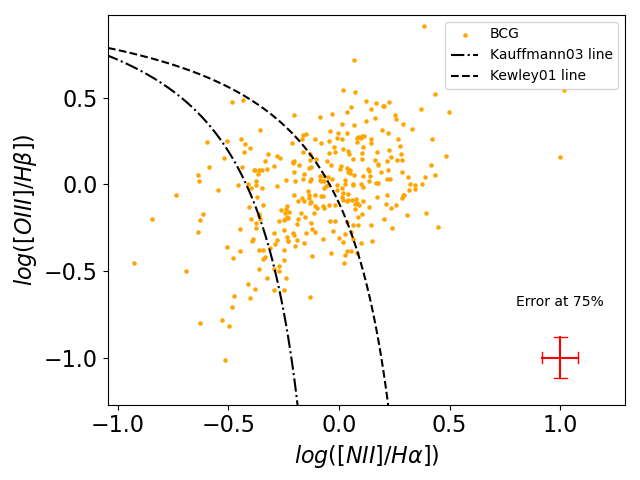
\includegraphics[width=0.85\textwidth]{BCG-NII-V22}
  \caption{BPT diagnostic diagram [NII] for the BCG sample with demarcation lines according to \cite{2006MNRAS.372..961K}.
  Additionally, a cross is placed to represent the 75th percentile of the error distribution for all points in the diagram.  }
  \label{4}
\end{figure}

\begin{figure}[hbtp]
  \centering
  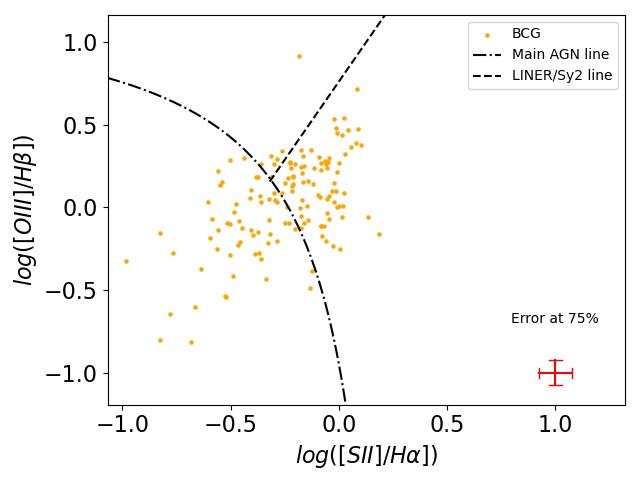
\includegraphics[width=0.85\textwidth]{BCG-SII1731-V22}
  \caption{BPT diagnostic diagram [SII] for the BCG sample with demarcation lines according to \cite{2006MNRAS.372..961K}.
  Additionally, a cross is placed to represent the 75th percentile of the error distribution for all points in the diagram. }
  \label{5}
\end{figure}


\begin{figure}[hbtp]
  \centering
  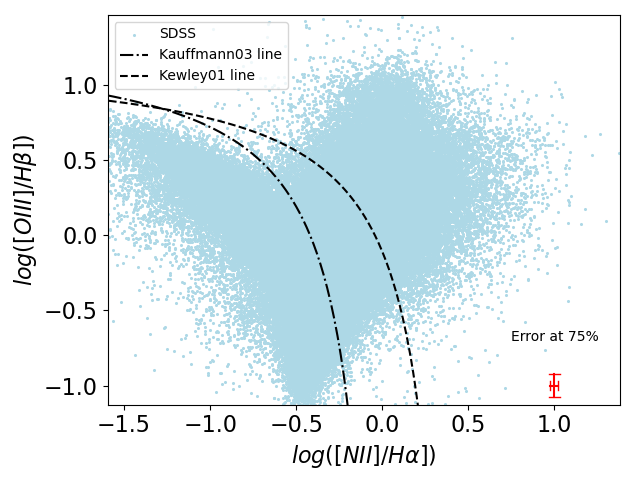
\includegraphics[width=0.85\textwidth]{SDSS-NII-V22}
  \caption{BPT diagnostic diagram [NII] for the non-BCG sample with demarcation lines according to \cite{2006MNRAS.372..961K}.
  Additionally, a cross is placed to represent the 75th percentile of the error distribution for all points in the diagram. }
  \label{6}
\end{figure}

\begin{figure}[hbtp]
  \centering
  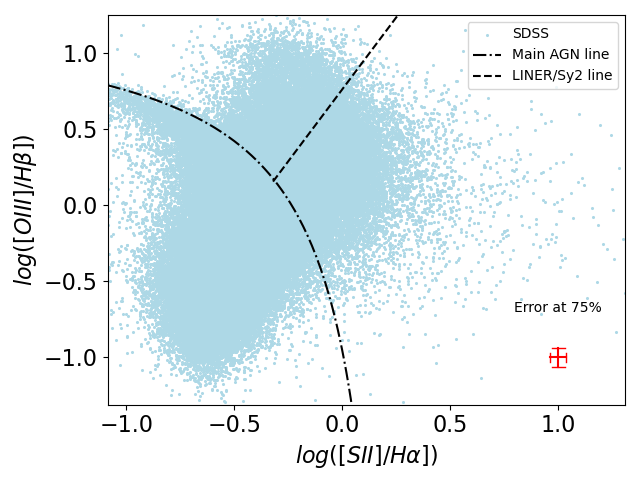
\includegraphics[width=0.85\textwidth]{SDSS-SII1731-V22}
  \caption{BPT diagnostic diagram [SII] for the non-BCG sample with demarcation lines according to \cite{2006MNRAS.372..961K}.
  Additionally, a cross is placed to represent the 75th percentile of the error distribution for all points in the diagram. }
  \label{7}
\end{figure}


\newpage
\subsection{Radio AGN activity in BCG and non-BCG galaxies}
In this analysis I use the catalog from Best et al. \cite{2005MNRAS.362....9B} based on observations from NVSS and FIRST surveys, to estimate the fraction of BCGs and non-BCGs galaxies exhibiting radio emission due to AGN activity.
A crucial step in calculating a representative fraction of Radio Loud objects was to appropriately define the spatial regions for the fraction calculations. To accomplish this, I identified the regions mapped by the radio survey employed. Subsequently, the selection has been delineated in the overlap of the three catalogs employed in this study. It is essential to emphasize that the primary objective is to obtain representative fractions of radio loud activity for the galaxies in both samples.
Based on the previously explained details regarding the precision of the Radio survey, galaxies displaying radio loudness were selected from the SDSS dataset within a distance of less than 5 arcseconds, equivalent to the beam size of the radio observations. This process resulted in two distinct samples, each containing both spectral properties and radio loud detections, for a total of 409 and 365,666 galaxies identified as BCG and non-BCG, respectively. In Fig.\ref{8}, I report the refined spatial regions required for determining the radio loud fractions, along with a visual representation of the BCGs and the radio emitters identified through cross-matching the catalogues.

\begin{figure}[hbtp]
  \centering
  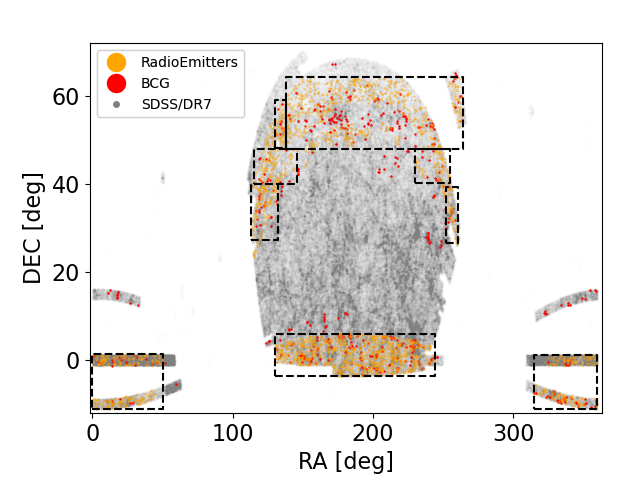
\includegraphics[width=0.95\textwidth]{Fourth}
  \caption{Distribution of data on the sky in J2000 Equatorial Coordinates. The grey areas depict galaxies included in the main sample \cite{mpa-sdss-dr7}, while BCGs identified through crossmatching are highlighted in red. Sources of radio emission found by Best et al. \cite{2005MNRAS.362....9B} are shown in orange. Dashed lines delineate the sky regions where the calculation of Radio Loud AGN fractions has been defined. }
  \label{8}
\end{figure}

\begin{comment}
To do a reasonable comparison between these fractions i need to cross-match the area obtained from the previous cross-match, between SDSS and the C4 BCG catalogue with the radio survey adopted. In Fig.\ref{8} I report the distribution of galaxies from SDSS DR7 in grey and the BCGs identified from the crossmatch in red. Galaxies covered from Best et al. detections is represented in orange. The black dashed squares show the refined cross-matched area used to produce the BCG and non-BCG samples.
From this procedure is selected two catalogs of “BCG” and “non-BCG” within the new cross-matched area, and flagged elements that show radio loud emission as reported by the radio survey from Best et al.
In these two new sub-samples I selected the galaxies associated to a radio-loud source in the radio catalog.

Based on the previously explained details regarding Radio survey's precision, galaxies displaying radio loudness were selected from the SDSS dataset within a distance of less than 5 arcsec. 

At the end, through this process, i obtained two distinct samples, each containing both spectral properties and radio loud detections, for a total of 409 and 365666 galaxies identified as BCG and non-BCG, respectively. In Fig.\ref{8} i report the refined space regions needed for the determination of the radio loud fractions, together with a visual depiction of the BCGs and the Radio Emitters identified by cross-matching the catalogues. 



A crucial step in calculating a representative fraction of Radio Loud objects was to appropriately define the spatial regions for the fraction calculations. To accomplish this, I identified the regions mapped by the radio survey employed. Subsequently, the selection has been delineated where all three catalogs exhibited an overlap. It is essential to emphasize that the primary objective is to obtain representative fractions for both of our samples.
\end{comment}





 
    
\chapter{Results}
Table \ref{tab:Optical2} shows the fractions estimated from the analysis of the BPT diagnostic diagrams for the two samples collecting galaxies selected as BCG and non-BCG, according to the selection on signal-to-noise ratio (SNR) greater than 3 and aligning non-BCGs to the same redshift range as BCGs. This filtering resulted in a set of 149 and 78 galaxies, respectively, for the BPT-[NII] and BPT-[SII] diagrams in the BCG sample. In the same context, there were 98,571 and 88,867 galaxies for the non-BCG sample.
To evaluate AGN activity, particularly in the BPT-[SII] diagnostic diagram, the combination of the Seyfert and LINER categories allows a further estimation of the maximum percentage. Analyzing the results presented in Table \ref{tab:Optical2} , the fraction of AGN in the BCGs sample range from 58$\%$ to 74$\%$. In the corresponding context, non-BCGs exhibit percentages in the range of 12$\%$ to 13$\%$. These values are consistent with the findings of \cite{2012A&A...546A..17V}, even if the results they report are derived from a larger sample that includes BCGs and sources with a SNR also lower than 3.
This calculations indeed show that BCGs show a greater optical AGN fraction, than non BCGs.
A further analysis was also implemented by dividing the BCG sample into four bins with the same number of elements and calculating the AGN fractions for both samples in relation to these bins.
Results of the latter, depicted in Fig.\ref{IMG:frac_z}, suggest that although the AGN fraction for non-BCGs shows a slight increase within the redshift range of BCGs (i.e., $0.02 \leq z \leq 0.1$), the corresponding percentages for BCGs remain constant at a value of 65/70$\%$, as depicted in Fig.\ref{IMG:frac_z}. Such an increase could not be detected with these calculations in the BCG sample, due to both smaller statistics and a broader dispersion of errors, but these results cannot exclude it. In this context, for future developments, it would be interesting to analyze the reasons behind the broader dispersion of errors for the fraction of non-BCGs at lower redshift.

Lastly, the analysis dedicated for detecting the BCGs and non-BCGs associated with radio loud emission indicates that BCGs are more likely to host radio luminosity exceeding 5mJy at 1.4 GHz, with a fraction of $12\%$. This value is 20 times higher than the fraction found for the non-BCG subsample of galaxies within the selected regions, as discussed earlier, corresponding to $0.6\%$.

%COSE TENUTE PER SICUREZZA MA MIGLIORATE E DUNQUE DEPRECATE !
\begin{comment}

 The additional selection in redshift significantly altered the information captured by the census of both samples. Specifically, within BCGs in Table \ref{tab:Optical}, the vast majority of species are at least suspected to host an AGN, rather than exhibiting prevalent star-forming characteristics. However, when looking at the same values in Table \ref{tab:Optical2}, the suspicion becomes almost a certainty.
Meanwhile, the BPT-[SII] analysis goes further, defining the main feedback coming from such AGNs. It is evident in Tables \ref{tab:Optical} and \ref{tab:Optical2} that the main population of AGNs shows low ionization ratios.
This change, resulting from the further selection in redshift, also alters the information obtained from non-BCGs census. Initially, the BPT-[SII] findings indicate that most objects detected as Composite appear to be star-forming galaxies. However, with the subsequent selection in redshift, this assumption becomes less certain, leading to a better subdivision between Liners and SF galaxies.

In \ref{tab:Optical}, detailing the results of the optical analysis, it is observed that BCGs are more likely to host an AGN compared to ordinary galaxies. Percentages obtained for the non-BCG sample are consistent with Vitale et al. \cite{2012A&A...546A..17V}. 

It is noteworthy that the percentages obtained for the non-BCG sample align with the findings of Vitale et al. \cite{2012A&A...546A..17V}. This observation leads to the conclusion that BCGs are more likely to exhibit AGN activity, as discussed in the previous context of percentages.

\begin{table}[htb]
  \centering
  \begin{tabular}{cccc}
    \hline\hline
    \multicolumn{1}{c}{Diagram} & Classification & non-BCG & BCG \\
    \hline
    [NII]  & AGNs &  $52896 \pm 84$ ($21.1 \pm 0.03$)$\%$ &$161 \pm 5$ ($50.4 \pm 1.6$)$\%$ \\
           & Composites & $55875 \pm 110$ ($22.3 \pm 0.04$)$\%$ & $110 \pm 5$ ($34.5 \pm 1.8$)$\%$ \\
           & SFGs & $141753 \pm 80$ ($56.6 \pm 0.03$)$\%$ &$ 49 \pm 4$ ($15.4 \pm 1.4$)$\%$ \\ 
    \hline
    [SII]  & Seyferts & $13082 \pm 64$ ($6.3 \pm 0.03$)$\%$  &$8 \pm 2$ ($6.5 \pm 1.6$)$\%$\\
           & LINERs & $28396 \pm 80$ ($13.6 \pm 0.04$)$\%$ & $74 \pm 3$ ($53.3 \pm 2.4$)$\%$ \\
           & SFGs &$167826\pm 76 $ ($80.2 \pm 0.04$)$\%$ & $55 \pm 3$ ($40.2 \pm 2.2$)$\%$\\ 
    \hline\hline
  \end{tabular}
  \caption{Results of the classification using BPT diagnostic diagrams, according to the criteria established by Kewley et al. \cite{2006MNRAS.372..961K}. The outcomes are presented in terms of counts per region and as a percentage for each population. }
  \label{tab:Optical}
\end{table}

\end{comment}
%Da riportare nel testo !!!!!!!!
%PER BCG NII ci sono 149
%PER BCG SII ci sono 78
%PER NON NII ci sono 98'571
%PER NON SII 88'867
\begin{table}[htb]
  \centering
  \begin{tabular}{cccc}
    \hline\hline
    \multicolumn{1}{c}{Diagram} & Classification & non-BCG & BCG \\
    \hline
    [NII]  & AGNs & $12.04 \pm 0.03$ $\%$ & $58.0 \pm 1.8$ $\%$ \\
           & Composites & $17.49 \pm 0.05$ $\%$ &  $34.7 \pm 2.2$ $\%$ \\
           & SFGs & $70.47 \pm 0.03$ $\%$ &  $7.3 \pm 0.2$ $\%$ \\ 
    \hline
    [SII]  & Seyferts & $4.22 \pm 0.03$ $\%$  & $6.6 \pm 1.7$ $\%$\\
           & LINERs & $9.03 \pm 0.04$ $\%$  & $67.6 \pm 2.5$ $\%$\\
           & SFGs &$86.75 \pm 0.04$ $\%$  & $25.9 \pm 2.1$ $\%$\\
    \hline\hline
  \end{tabular}
  \caption{Results of the classification using BPT diagnostic diagrams, following the criteria established by Kewley et al. \cite{2006MNRAS.372..961K}. The samples were additionally refined by requiring a signal-to-noise ratio (SNR) greater than 3 and aligning non-BCGs within the same redshift range as BCGs. The results are presented as percentages for each population. }
  \label{tab:Optical2}
\end{table}

\begin{figure}[t]
  \centering
  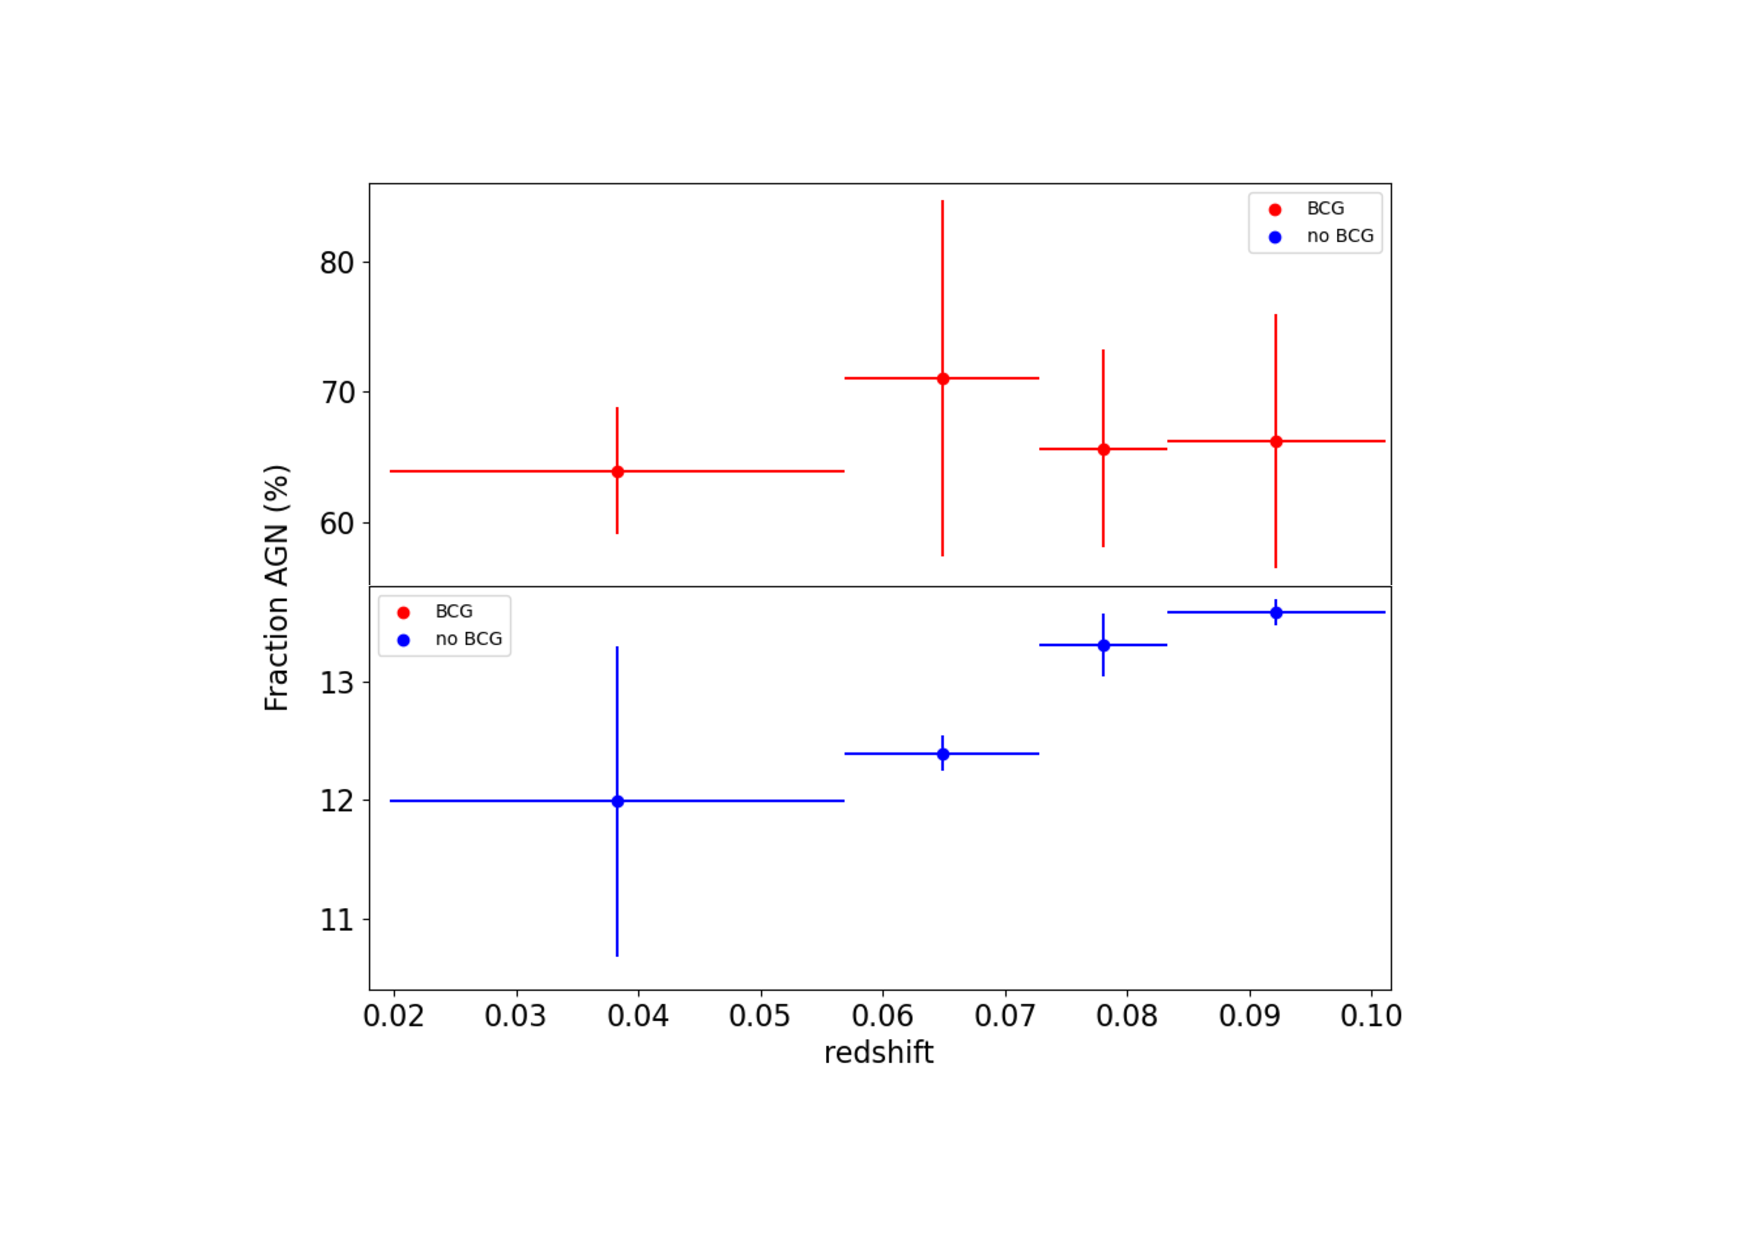
\includegraphics[width=0.85\textwidth]{zfractionAGN}
  \caption{Visual representation illustrating the absence of redshift fluctuation in AGN activity percentages, specifically as AGN in the BPT [NII] diagnostic diagram and as Seyfert + LINER in the BPT [SII] diagnostic diagram. Redshift bins are uniformly defined to maintain consistent BCG statistics within each bin. The samples underwent further refinement by imposing a signal-to-noise ratio (SNR) threshold greater than 3, and aligning non-BCGs within the identical redshift range as BCGs.}
  \label{IMG:frac_z}
\end{figure}

    
\chapter*{Conclusions}
\addcontentsline{toc}{chapter}{Conclusions}{}  % mette le conclusioni nell'indice

The final chapter of the thesis
is a summary of the work done.
Therefore, in its first part it resembles much the introduction,
adding to it the actual result of the work,
its future evolution and prospects,
in the view of the writer. 

\bibliographystyle{plainnat}
%\setcitestyle{authoryear,open={(},close={)}}
\bibliography{articoli}{}


%% The bibliography contains all the bibliographic references presented in the text.

\begin{thebibliography}{99} % il 99 e' il massimo numero che ci si aspetta di leggere fra i riferimenti

\bibitem{NSS}
T.~Oetiker, H.~Partl, I.~Hyna, and E.~Schlegl,
``The Not So Short Introduction to \LaTeXe'',
https://tobi.oetiker.ch/lshort/lshort.pdf


\end{thebibliography}









         

% INIZIO COMMENTO
\begin{comment} 

% quello che sta qui non viene compilato

%\listoffigures

%\listoftables

\end{comment}
% FINE COMMENTO


\end{document}

